\documentclass[bachelor]{njupthesis}

\title{定向覆盖模糊测试工具的设计与实现}
\author{雷尚远}
\advisor{王子元}
\school{计算机学院、网络学院、网络空间安全学院}
\major{计算机科学与技术}
\studentclass{B190303}
\studentid{B19030334}
\graduateyear{2023}
\begindate{2023年3月x日}
\finishdate{2023年6月x日}


\begin{document}

\makecover

\begin{chineseabstract}
模糊测试(Fuzzing)是一种通过向目标系统提供非预期的输入并监视异常结果来发现软件安全漏洞的方法,
是软件安全领域常用的方法之一。由于代码覆盖率与漏洞覆盖率密切相关,大多数模糊测试工具都是
以代码覆盖率为导向。然而,由于大多数被覆盖测试的代码可能并不包含漏洞,这使得盲目地扩展
代码覆盖率的方式在实际测试时效率较低。极端情况尤为如此。与盲目增加代码覆盖率的模糊测试不同,
定向覆盖的灰盒模糊测试(DGF)将大部分时间用于检测特定目标区域(例如,易出错代码段)而不会
浪费资源于不相关的部分。因此,DGF 特别适用于补丁测试、漏洞复现以及特殊漏洞检测等场景。
目前,DGF 已成为一个快速发展的研究方向。基于一些先进的定向覆盖模糊测试工具的研究和相关调查,本文
主要做了以下点工作:
\begin{enumerate}[label=(\arabic*)]
	\item 基于现有的模糊测试工具框架AFL(American Fuzzy Lop)以及AFLGo做了定向覆盖策略的设计和集成;
	\item 实现了简单的定向覆盖的模糊测试命令行工具;
	\item 针对相应的公开通用漏洞集(CVE)做了复现及定向实验对比测试。
\end{enumerate}
此外本文亦通过分析工具设计以及实现过程中的局限性与不足,对于未来该方向的研究发展做出了一些展望。

\chinesekeyword{模糊测试;定向覆盖模糊测试;灰盒测试;软件安全}
\end{chineseabstract}

\begin{englishabstract}
Fuzzing is a method of discovering software security vulnerabilities by providing 
unexpected inputs to a target system and monitoring for abnormal results. It is one of the 
commonly used methods in the field of software security. As code coverage is closely related 
to vulnerability coverage, most fuzz testing tools are guided by code coverage. However, blindly 
extending code coverage may be inefficient in practical testing since most of the covered code 
may not contain vulnerabilities, especially for corner cases.  In contrast to blind code coverage-based 
fuzz testing, directed grey-box fuzzing (DGF) spends most of its time detecting specific target regions 
(such as error-prone code segments) rather than wasting resources on irrelevant parts. 
Thus, DGF is particularly suitable for scenarios such as patch testing, bug reproduction, and 
special bug detection. For now, DGF has become a fast-growing research area.  Based on some advanced 
directed coverage fuzz testing tools and relevant investigations, this article mainly focuses on the 
following points of work:
\begin{enumerate}[label=(\arabic*)]
	\item Designed and integrated a directed coverage strategy based on the existing fuzzy testing tool framework AFL (American Fuzzy Lop) and AFLGo;
	\item Implemented a simple command-line tool for directed fuzz testing;
	\item conducted reproductions and directed experiments on corresponding public vulnerability databases (CVE) for comparative testing。
\end{enumerate}
In addition, this article also provides some prospects for the future research and development of this direction by 
analyzing the limitations and deficiencies in the design and implementation process of the tool.


\englishkeyword{Fuzzing;Directed Greybox Fuzzing;Greybox test;Software Security}
\end{englishabstract}

\thesistableofcontents

\thesischapterexordium

\chapter{绪论}


\section{背景分析}
\section{国内外研究现状}
\section{研究内容}
\section{论文结构}

\chapter{相关技术研究}
\section{模糊测试技术}
\subsection{黑盒模糊测试技术}
\subsection{白盒模糊测试技术}
\subsection{灰盒模糊测试技术}
\section{定向模糊测试技术}
\subsection{白盒定向模糊测试技术}
\subsection{灰盒定向模糊测试技术}
\section{研究动机}
\section{本章小结}

\chapter{基于AFLGo的定向模糊测试策略集成}
\section{模糊测试技术}
\subsection{黑盒模糊测试技术}
\subsection{白盒模糊测试技术}
\subsection{灰盒模糊测试技术}
\section{定向模糊测试技术}
\subsection{白盒定向模糊测试技术}
\subsection{灰盒定向模糊测试技术}
\section{研究动机}
\section{本章小结}




 这是一个参考文献示例\cite{PRODEN}

% \section{Apple M1}
% 这是一个公式
% \begin{equation}
% 	y=A x+b
% \end{equation}


% \subsection{名字自己替换}
% 1994年12月,中国国务院批准开展京沪高速铁路预可行性研究。铁道部开展京沪高铁选线,提出“北线方案”,即从上元门地区,通过隧道过江。南京的规划部门则拿出“南线方案”,从大胜关过江。铁道部牵头,进行比选得出的结论是:两个方案在技术上都可行,主要差别在于工程造价、经济效益、运营条件等方面。江苏省和南京市要求南线方案,而铁道部看好的始终是北线方案。南京力主南线,是放长了眼光。如果从南京北部走,已经不具备扩建条件。南京火车站虽然前面是玄武湖、背面是小红山,景观很美,但是已经没有拓展空间。此外,更重要的是,在全国任何一个城市,铁路带动城市发展的效果都非常明显,南京要想进一步发展南部区域,这是个好机会。显然,高铁建在哪里,也就意味着南京今后的发展框架,是继续囿于老城狭小的空间里,还是大步向南拓展。铁道部青睐北线的理由:新线与既有线的衔接方便。清末修建的津浦铁路,即从天津到浦口;在长江南岸,之后又修建了沪宁铁路。浦口火车站、下关火车站、南京站,南京重要的火车站,向来都是位于城北。并且,当时铁道部的人都认为,南京的城市中心就在北边。另一方面,铁路的机务段、职工宿舍等都在城北,建成之后,职工上下班都方便。为了说服铁道部,南京方面列出了南线的九大优势:无论高铁从哪里走,从完善南京枢纽总体布局的角度来看,都必须建大胜关长江大桥;根据国务院批准的南京城市规划,南京城市今后将主要向东南方向发展,大胜关方案符合城市扩展方向;南面的场站位置已预留多年,有较为理想的建站条件;沿线拆迁量小,对城市干扰和环境影响小;利于形成方便的铁路——航空换乘及铁路与城市道路联结条件……不过,这些最初并没有打动铁道部,铁道部仍然坚持北线方,双方为此对峙了好几年。


% \subsection{名字自己替换}
% 1995年,为了促进高铁尽快上马,南京稍稍“松口”。在当年的一份紧急报告里,有这样一句话——“南北方案之争不宜过多坚持,而从规划上对北线方案提出完善意见为妥”。南京市规划局做了两手准备,针对南线、北线方案,分别做了规划控制。从1995年起,南京根据两个方案,开始分别严格控制沿线用地建设,同时冻结了南北两条线周围的土地。而这个具有预见性的做法,使得后来的工作变得轻松许多。

% 南京南站如图\ref{南京南站}所示。
% \begin{figure}[hbt]
% 	\centering
% 	\subfigure[南京南1]{
% 		\begin{minipage}[b]{0.4\textwidth}
% 			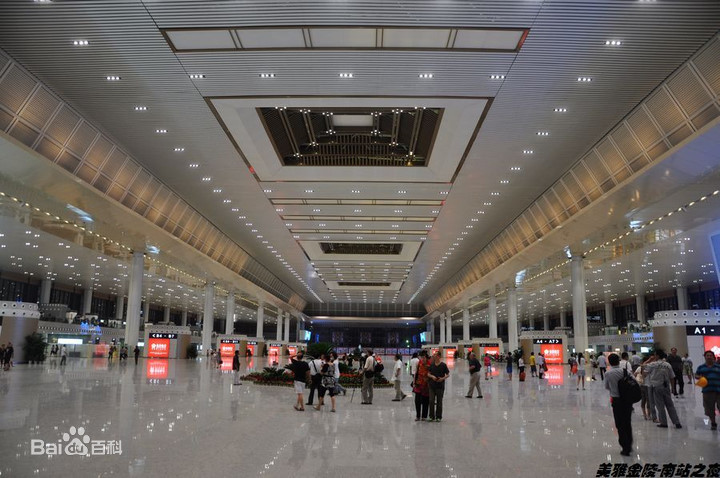
\includegraphics[width=1\textwidth]{1}
% 		\end{minipage}
% 	}
% 	\subfigure[南京南2]{
% 		\begin{minipage}[b]{0.4\textwidth}
% 			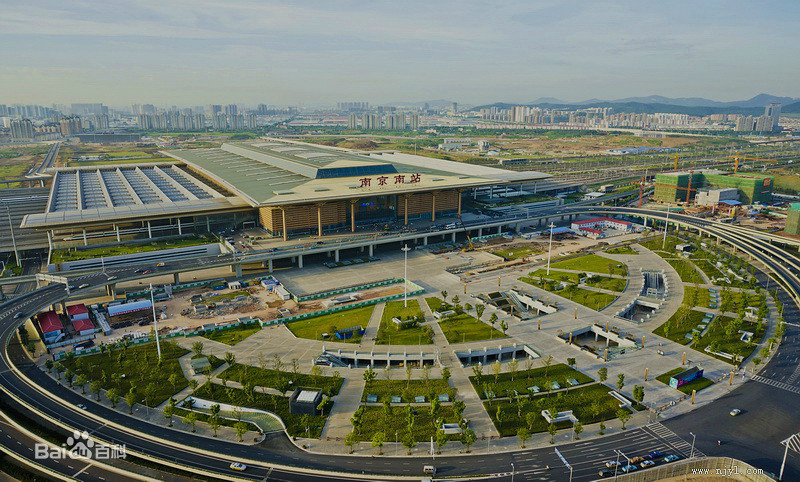
\includegraphics[width=1\textwidth]{2}
			
% 		\end{minipage}
% 	} \\
% 	\subfigure[南京南3]{
% 		\begin{minipage}[b]{0.4\textwidth}
% 			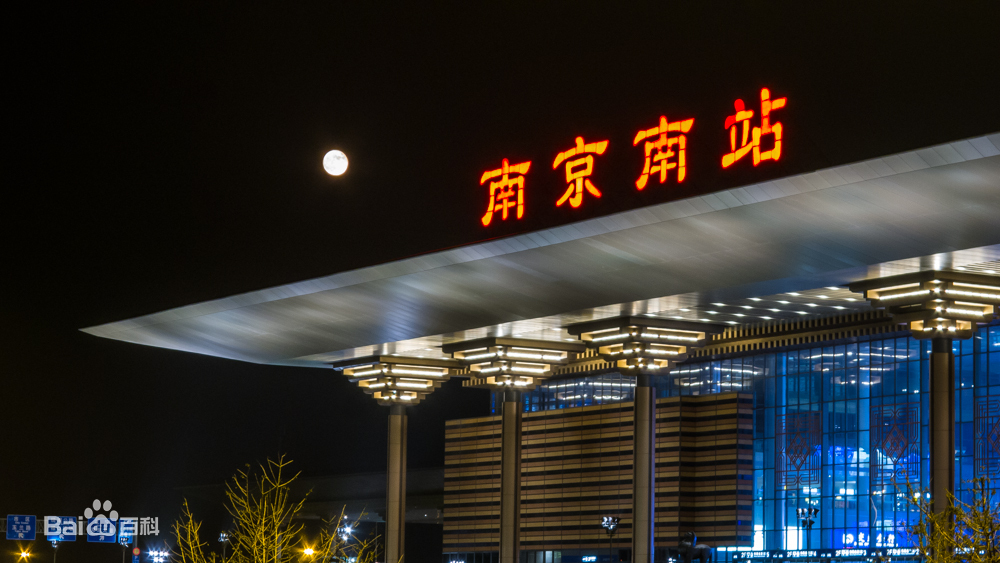
\includegraphics[width=1\textwidth]{3}
% 		\end{minipage}
% 	}
% 	\subfigure[南京南4]{
% 		\begin{minipage}[b]{0.4\textwidth}
% 			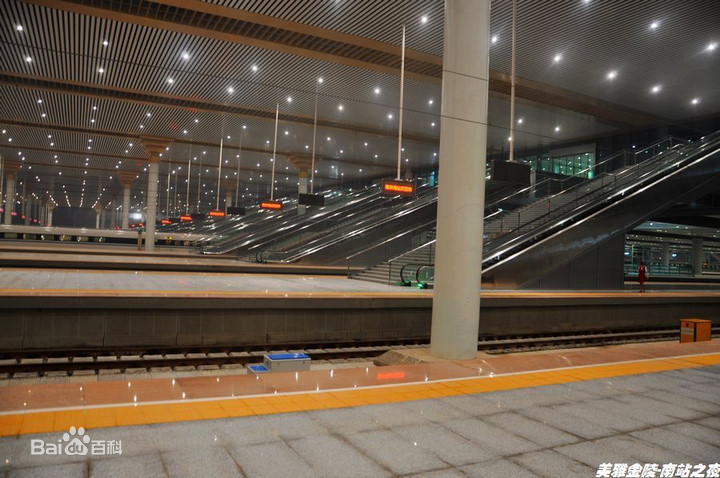
\includegraphics[width=1\textwidth]{4}
			
% 		\end{minipage}
% 	}
% 	\caption{南京南站}
% 	\label{南京南站}
% \end{figure}


\chapter{需要几章自己加一下!}

%这里是结束语
\thesisconclusion

% 致谢区域
\thesisacknowledgement

本论文采用\LaTeX 模版编写的,是基于南京邮电大学2021年理工艺教类的Word模板进行严格迁移编写的。本模板地址\url{https://github.com/dhiyu/NJUPT-Bachelor}感谢imguozr(\url{https://github.com/imguozr/NJUPThesis-Bachelor} )和lemoxiao(\url{https://github.com/lemoxiao/NJUPThesis-Scholar} )的工作,为本模板的形成奠定了大量的基础。

% 参考文献区域
\thesisreference

%附录区域
\thesisappendix

\section{本科期间的学术成果发表情况}
\begin{itemize}
	\item 发表一篇Nature
	\item 获得了诺贝尔奖
	\item 当选足球先生
	\item 开发了1nm光刻机一台
\end{itemize}

\section{本科期间的获奖情况}
\begin{itemize}
	\item 设计了一块RTX5090
	\item 准备移民火星
	\item 去太阳上面看看
\end{itemize}

\end{document}